% !TEX root = ../main.tex
%
\chapter{Dibaryons} \label{sec:2}

\cleanchapterquote{I think I can safely say that nobody understands quantum mechanics.}{Richard P. Feynman}{(The Character of Physical Law)}


The term dibaryon denotes any object with baryon number B = 2. In this sense the first known dibaryon
has been the deuteron discovered in 1932~\cite{deu_disc}.
In terms of quarks a dibaryon is a composed state of six valence quarks.
It may be of molecular type, i.e. spatially extended with two well separated interacting quark 
bags as is the case of the deuteron. Or \ -- more exotic and hence more interesting -- \ a dibaryon
could be a spatially compact hexaquark object, where all six quarks are confined in a single quark bag.

The dibaryon searches have started in the fifties and have been very changeful, with many 
successes and failures. 
Early predictions of a vast number of dibaryon states initiated endless experimental claims,
but finally none survived careful experimental investigations. 

Despite their long history dibaryon searches have recently received renewed interest,
in particular by the recognition that there are more complex quark configurations than just the 
well known $q\bar{q}$ and $qqq$ systems \ -- e.g. the LHCb observation of a pentaquark 
state~\cite{lhcbpenta}.
The WASA-at-COSY collaboration has found that the double-pionic fusion reaction $pn \rightarrow 
d \pi^{0} \pi^{0}$ proceeds dominantly via a resonance structure observed in the total cross section 
at $\sqrt{s} = 2.37\ $ GeV~\cite{wasa1}. 


Nearly all possible decay channels have been investigated~\cite{wasa2, wasa3, wasa4}.
New data on polarised neutron-proton scattering in the region of interest exhibit a resonance pole in 
the partial waves analysis in accordance with the resonance hypothesis~\cite{wasa5,wasa6}.
This provides the first solid evidence for the existence of a non-trivial dibaryon.

Since the measurements suggest this resonance to decay dominantly via an intermediate $\Delta \Delta$
system, it constitutes asymptotically a $\Delta \Delta$ system bound by nearly 100 MeV \ -- as 
predicted by Dyson and Xuong~\cite{dysonxuong} already in 1964.
Furthermore, most recent relativistic three-body calculations based on hadron dynamics~\cite{haddin}
as well as quark model calculations~\cite{dsqm1,dsqm2} succeeded to predict properly a number
of characteristics of this resonance.

%
%
\section{Dibaryon binding mechanism} \label{sec:2.1}

In 1977 Jaffe predicted the existence of the so-called $H$ dibaryon, a hadronically bound 
$\Lambda \Lambda$ system containing two strange quarks.
After the Jaffe work, many other theoretical predictions of dibaryons appeared in the following years. 
They were based on QCD-inspired models like bag, potential, string or flux-tube models for the
six-quark system~\cite{dsinevitable1,dibpred1,dibpred2,dibpred3,dibpred5,dibpred6,dibpred7,dibpred8,
dibpred9,dibpred10,dibpred11,dibpred12,dibpred13}.
Other models were based on the hadronic baryon–baryon interaction without any explicit quark degrees
of freedom~\cite{dibpred14,dibpred15,dibpred16} or just symmetry considerations based on SU(3)
~\cite{dibpred17}.

%
% \subsection{QCD-inspired models} \label{sec:2.1.1}

In general, the QCD-inspired model calculations are based on the colour-magnetic interaction between 
quarks giving rise to hyperfine splitting:
\begin{equation} \label{eq:colmag}
    v_{colour-mag} = - \sum_{i<j} (\lambda_{i} \cdot \lambda_{j}) (\sigma_{i} \cdot \sigma_{j})
    v(r_{ij})
\end{equation}
where $\lambda_{i}$ and $\sigma_{i}$ denote colour and spin operators, respectively, of the quark $i$, 
while $v(r_{ij})$ is a flavor conserving short-range interaction between the quarks i and 
j~\cite{colormag}.
As shown by Jaffe, the colour-magnetic interaction is most attractive in the flavor-singlet state with
$I(J^{P}) = 0(0^{+})$ and $S = -2$, that represent the $H$ dibaryon. The wavefunction of this state
correspond, asymptotically, to baryon-baryon configurations of $\Lambda \Lambda$, $\Xi N$ and 
$\Sigma \Sigma$~\cite{oka}. In this picture the leading dibaryon candidates, having the underlying 
baryons in relative S wave are the following states:
\begin{itemize}
    \item $S=0 \ $, $I(J^{P}) = 0(3^{+})$ and BB structure $\Delta \Delta$,
    \item $S=-1\ $, $I(J^{P}) = 1/2(2^{+})$ and BB structure $\Sigma^{*}N$ and $\Sigma \Delta$,
    \item $S=-2\ $, $I(J^{P}) = 0(0^{+})$ and BB structure $\Lambda \Lambda$, $\Xi N$ and 
$\Sigma \Sigma$ \ -- the $H$ dibaryon,
    \item $S=-3\ $, $I(J^{P}) = 1/2(2^{+})$ and BB structure $\Omega N$, $\Xi^{*} \Sigma$, 
    $\Xi \Lambda^{*}$ and $\Xi \Sigma^{*}$,
\end{itemize}
where BB means the baryon–baryon configuration, which is asymptotically closest to the dibaryon
state.

The results based on Equation~\ref{eq:colmag} assume unbroken SU(3) symmetry.
However, more realistic models, which account for symmetry breaking, lead to significant changes
in the predicted dibaryon masses.
With respect to a possible experimental observation of dibaryon resonances, predictions of states
with low masses are particular interesting because of their expected narrow width that are easier
to observe.

Other models are based on the partial-wave analyses of $NN$ scattering.
introducing an elongated quark bag allowing for finite orbital angular momenta between
delocalised quark clusters in the partitions $q^{2}-q^{4}$ and $q-q^{5}$. 
These models derive and effective potential \ -- as the Nijmegen 
potential~\cite{dibpred1,dibpred2,dibpred3} -- \ predicting a multitude of dibaryon resonances
both in non-strange and strange sectors. 

The Los Alamos theory group predicted dibaryons in the $\Omega N$ system, which could be so
deeply bound that they would be stable with respect to strong 
decay~\cite{dsinevitable1,dsinevitable2}.
They also showed that predictions about the binding energy of the dibaryons critically depend
on the detailed dynamics of the model under consideration.

Recently the question, whether the H dibaryon is bound or not, has been addressed by two 
state-of-the-art lattice QCD calculations~\cite{Hlattice1,Hlattice2} obtaining
that the $H$ dibaryon to be bound by about 8 MeV.
Subsequent theoretical investigations show that such predictions require still quite some
fine-tuning~\cite{Hlattice3}.

The prediction of a copious number of dibaryon states in strange and non-strange sectors 
initiated a rush of experimental searches for such states. 
The importance of the observation of these states lies in the possibility to discriminate
between the multitude of models that try to describe the baryon-baryon binding mechanism.
Furthermore, this subject is connected to the low energy quark-quark interaction problem,
therefore the characterisation of these very interesting objects can improve our 
understanding of the non-perturbative QCD.

%
%
\section{The \dst dibaryon} \label{sec:2.2}

The \ds dibaryon \ -- or more accurately \dst -- \ is the main subject of this thesis.
It has been observed for the first time \ as already mentioned -- \ by the WASA-at-COSY 
collaboration in 2011~\cite{wasa1}.
Event though this observation is based on solid experimental evidence, it needs an independent
confirmation, since in the past all the dibaryon discovery claims have never been confirmed.
In this section more details about the \ds dibaryon, from the early predictions to the 
recent experimental observation are given.

%
\subsection{Predictions} \label{sec:2.2.1}

The first prediction of the existence of this state dates back to 1964. 
It had become apparent, at that time, that baryons and mesons contain substructures, the quarks.
The QCD does not prohibit colorless multiples of three quarks, in particular does not forbid 
quarks in a colorless six-pack. In fact Dyson and Xuong~\cite{dysonxuong} demonstrated that SU(6)
symmetry provides a multiplet of six non-strange dibaryon states denoted by $D_{IJ}$ 
(See Tab.~\ref{tab:dibaryons}).

\begingroup
\renewcommand{\arraystretch}{1.2} % Default value: 1
\begin{table}
\centering
\begin{tabularx}{\textwidth}{cXXlc}
% \textbf{The Dyson multiplet}
\toprule
\textbf{Notation}    &   \textbf{I}   &   \textbf{J}   &   \textbf{Asymptotic baryon-baryon configuration}            &\textbf{Mass (MeV)} \\
\midrule
$D_{01}$    &   0   &   1   &   \qquad \qquad Deuteron                            &   1876    \\
$D_{10}$    &   1   &   0   &   \qquad \qquad $^{1}S_{0}\ NN$ virtual state       &   1876    \\ 
$D_{12}$    &   1   &   2   &   \qquad \qquad $\Delta N$                          &   2160    \\
$D_{21}$    &   2   &   1   &   \qquad \qquad $\Delta N$                          &   2160    \\
$D_{03}$    &   0   &   3   &   \qquad \qquad $\Delta \Delta$                     &   2350    \\
$D_{30}$    &   3   &   0   &   \qquad \qquad $\Delta \Delta$                     &   2350    \\
\bottomrule
\end{tabularx}
\caption{Prediction of Dyson and Xuong~\cite{dysonxuong} about a sextet of non-strange dibaryon states based on SU (6) symmetry. The states are denoted by $D_{IJ}$, where $I$ denotes the isospin and $J$ the total spin of the state. The associated asymptotic baryon–baryon (BB) configurations and the masses calculated from symmetry breaking are given.}
\label{tab:dibaryons}
\end{table}
\endgroup

Dyson and Xuong identified the first three states of the sextex as the deuteron groundstate, the virtual
$^{1}S_{0}$ isovector state and an $I(J^{P}) = 1(2^{+})$ state for which first experimental indications
had been available already at that time.
Since the first two states have roughly the same mass they hypothesized isospin independent mass for the 
dibaryon of this multiplet and derived a mass formula to predict other masses.
According to the mass formula the dibaryon state $D_{03}$ is expected to be at 2350 MeV, 
i.e. about 110 MeV below the $\Delta \Delta$ threshold.

Due to its quantum numbers it should asymptotically \ -- i.e. at large distances as an intermediate
step in its decay or formation -- \ conform to an isoscalar $\Delta \Delta$configuration with
$I(J^{P}) = 0(3^{+})$. This mean is, basically, composed by two spin-aligned $\Delta$ particles
in relative $S$-wave.

Despite the Dyson prediction is based on a static model \ -- SU(6) flavour symmetry, the dynamic
of the system has not been considered -- \ and the simplicity of the mass formula, it is very 
impressive that predicted properly the now discovered state \dst at a mass remarkably close to the
experimentally observed one. 
Subsequent, partially very complex theoretical investigations, turned out to be much less successful.
In particular they predicted often a multitude of states in addition, which were never observed.

Goldman et al.~\cite{dsinevitable1} \ -- members of the Los Alamos theory group -- \ in 1989 emphasised
the particular importance of the \textit{"inevitable"} \ds dibaryon, as they called it.
They also argued that certain basic features common to all models based on one-gluon exchange
and confinement lead unavoidably to the prediction of a non-strange dibaryon resonance \ds 
with $I(J^{P}) = 0(3^{+})$ due to its special symmetry.
In the Los Alamos calculations it appears to be very deeply bound by nearly 400 MeV.
In contrast, the MIT and cloudy bag model calculations~\cite{dibpred2,dibpred5,dibpred6}
obtained for it binding energies relative to the
$\Delta \Delta$ threshold of about 100 MeV.
Only recently \ -- after the experimental observation -- \ the calculations of this group approached
the experimental value in the framework of the so-called quark delocalization and colour screening model
(QDCSM)~\cite{dsqm1}.

Also the Nijmegen group~\cite{dibpred1,dibpred2,dibpred3} as well as Saito~\cite{dibpred6} predicted
this state correctly at the proper mass in their bag-model calculations. Only, they simultaneously predicted
within the same framework numerous other dibaryon states, which were never observed.

A correct real prediction \ -- i.e. a prediction before the experimental discovery of \dst -- \ was done 
by the IHEP theory group led by Z.Y. Zhang, who studied this state in the chiral SU(3) quark model within
the framework of the resonating group method (RGM)~\cite{dsqm2}.

A relativistic Faddeev-type calculation based on hadronic interactions have been reported by Gal and Garcilazo
recently to see this state, correctly at the experimental mass~\cite{reanalysis,haddin,haddin1}. 
It should be noted that those calculations give the same sequence of dibaryon states as predicted previously by 
Dyson and Xuong~\cite{dysonxuong}.

The prediction of the the decay width of the \dst is even more demanding than the prediction of the mass, since
it requires also a theoretical treatment of the dynamics of the decay process.
So far there are only three theoretical predictions for the decay width based either on Faddeev
calculations~\cite{reanalysis,haddin,haddin1} or on quark-model calculations within the
QDCSM  framework~\cite{widthpred1,dsqm1} and the RGM-based chiral SU(3) 
model~\cite{widthpred2,widthpred3}, respectively.

%
\subsection{Observations} \label{sec:2.2.2}

In the last years the WASA collaboration started to investigate the double-pionic fusion reaction 
$pn \rightarrow d \pi \pi$ in order to solve the puzzle of the ABC effect~\cite{abc} \ -- basically
a low-mass enhancement in the spectrum of the $\pi \pi$ invariant mass -- \ that occurs in this
reaction.
The idea is that the ABC effect could be a manifestation of a resonance, whose dominant asymptotic
configuration is a $\Delta \Delta$ system in relative $S$ wave: the \ds dibaryon.

In order to study the $pn \rightarrow d \pi \pi$ reaction the main problem is the source of
neutrons, since free neutrons are not available \ -- neither as beam or as target particles. 
Hence the quasi-free process with deuterons being the source for quasi-free neutrons has been utilised
by the WASA collaboration.
This process has the additional advantage that the Fermi motion of the neutron within the deuteron 
provides a range of collision energies with a single beam energy setting.
That way the energy dependence of a reaction can be conveniently scanned, which is particularly well
suited for the search for narrow resonances.
However, a precondition for a successful use of the quasi-free process is that the four-momenta of all
reaction products are determined experimentally, which necessitates exclusive and kinematically complete
measurements.
The WASA experiment was designed designed for this very purpose and the results about the measurement 
of the $pn \rightarrow d \pi^{0} \pi^{0}$ cross sections are reported in Figure~\ref{fig:wasares1}.

\begin{figure}
    \centering
    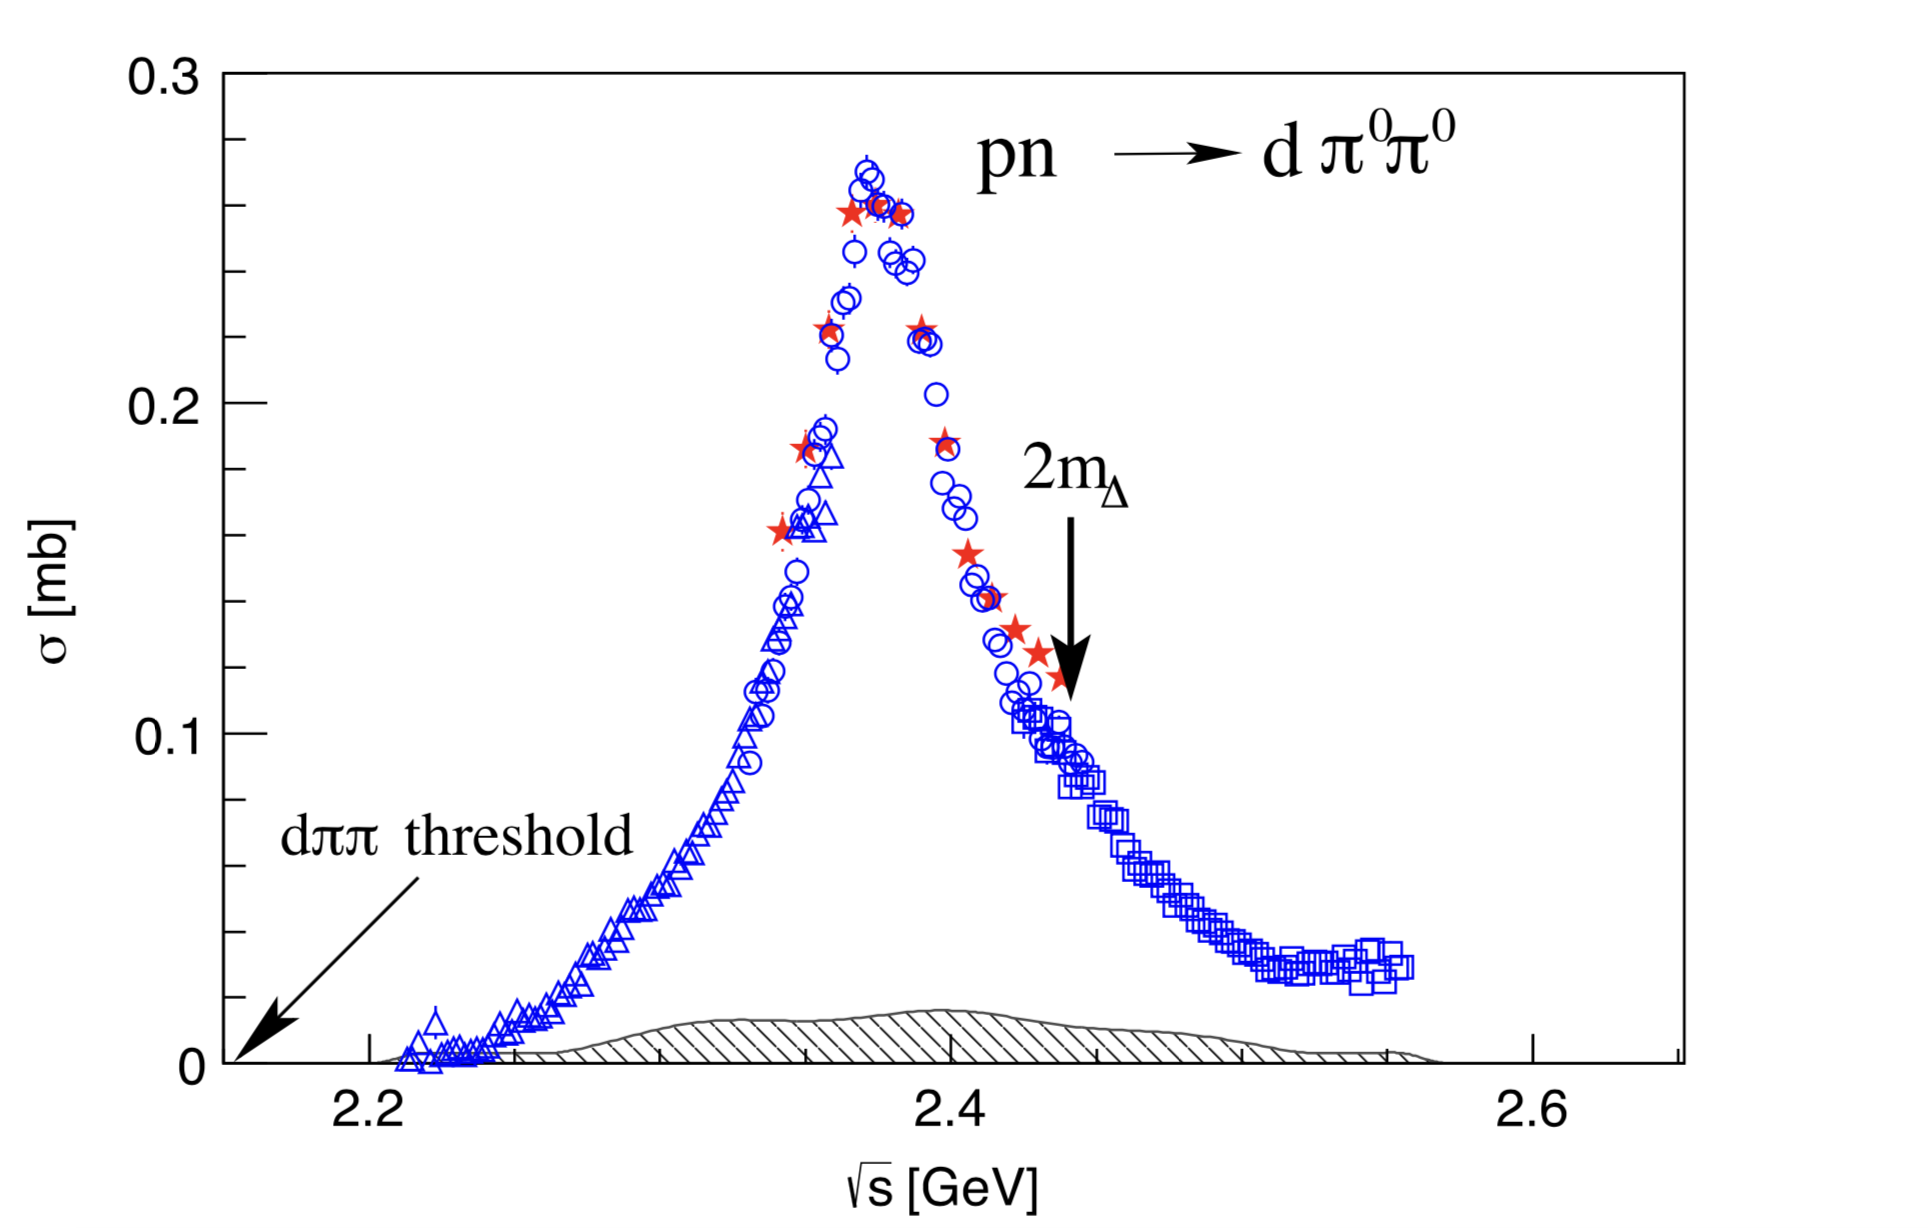
\includegraphics[width=0.9\textwidth]{gfx/wasares1}
	\caption{Measurements of the golden reaction channel $pn \rightarrow d \pi^{0} \pi^{0}$ with WASA at COSY. The total cross section exhibiting the pronounced resonance effect of \dst. The blue open symbols show the data of Ref.~\cite{wasa1} properly normalised in absolute scale to the data of Ref.~\ref{wasa2} plotted by red stars. The black shaded area gives an estimate of systematic uncertainties.}
	\label{fig:wasares1}
\end{figure}

The measurements of this reaction revealed a pronounced Lorentzian structure in the total cross section
corresponding to a resonance at $\sqrt{s} 2.37\;$ GeV with a width of $70\;$ MeV. 
The resonance structure is about 90 MeV below the mass of two $\Delta$ states and its width is more 
than three times narrower than that of a conventional t-channel $\Delta\Delta$ excitation.



% Fig. 11 shows the measurement of the total cross section as well as a selection of differential distributions at s = 2.38 GeV, the peak energy region. The shown data for the deuteron angular distribution (Fig. 11, on the left of the middle
% panel) are the result of two runs, one run with the spectator proton in the target, i.e., with the reaction pd → dπ 0 π 0 +pspectator (open circles), and another run with the spectator proton in the beam (reversed kinematics), i.e., with the reaction dp → pspectator + dπ0π0 (solid circles). That way the acceptance over the full angular range could be optimized. The data are in accordance with the Barshay–Temmer theorem [355], according to which the angular distribution of a purely isoscalar reaction has to be symmetric about 90° in the center-of-mass system. The dashed line shows a fit with an expansion into Legendre Polynomials of order = 0, 2, 4 and 6 corresponding to a total spin of the resonance of J = 3. Together with the fact that the pn → dπ 0 π 0 reaction is purely isoscalar, we get the quantum numbers I (J P ) = 0(3+ ) for this resonance structure. Due to its isoscalar character it is formally compatible with an excitation of the deuteron, hence it has been named d∗.
% In further WASA measurements it has been demonstrated that below and above this resonance structure the angular distributions get flatter [357]. The fact that the angular distribution flattens out towards lower energies is not unexpected, since towards the reaction threshold we expect contributions only from lowest partial waves. However, the observation that the angular distribution gets again flatter at higher energies is not trivial. It is in support of the fact that the high spin of J = 3 of the resonance requires an unusually large anisotropy of the angular distribution, which is larger than that of the conventional t-channel ∆∆ process, which dominates at higher energies



